\documentclass[11pt,a4paper]{ivoa}
\input tthdefs
\usepackage{float}

\usepackage{listings}
\lstloadlanguages{XML,java}
\lstset{flexiblecolumns=true,tagstyle=\ttfamily,
showstringspaces=False}

\title{A Component and Association Based Model for Source Data}

% see ivoatexDoc for what group names to use here
\ivoagroup{Data Model Working Group}

\author[http://wiki.ivoa.net/twiki/bin/view/IVOA/FrancoisBonnarel]{François Bonnarel}
\author[http://wiki.ivoa.net/twiki/bin/view/IVOA/TomDonaldson]{Tom Donaldson}
\author[http://wiki.ivoa.net/twiki/bin/view/IVOA/LaurentMichel]{Laurent Michel}
\author[http://wiki.ivoa.net/twiki/bin/view/IVOA/MarcoMolinaro]{Marco Molinaro}

\editor{Laurent Michel}

\previousversion{This is the first public release}
       

\begin{document}
\begin{abstract}
This note proposes a possible way to make source data interoperable. It takes into account the huge diversity of source data in term of both format and usage. Both data annotation and annotated data parsing processes are also considered in this document.
\end{abstract}


\section*{Acknowledgments}

Paris session speakers TDIG members

\section*{Conformance-related definitions}

The words ``MUST'', ``SHALL'', ``SHOULD'', ``MAY'', ``RECOMMENDED'', and
``OPTIONAL'' (in upper or lower case) used in this document are to be
interpreted as described in IETF standard RFC2119 \citep{std:RFC2119}.

The \emph{Virtual Observatory (VO)} is a
general term for a collection of federated resources that can be used
to conduct astronomical research, education, and outreach.
The \href{http://www.ivoa.net}{International
Virtual Observatory Alliance (IVOA)} is a global
collaboration of separately funded projects to develop standards and
infrastructure that enable VO applications.


\section{Introduction}

The source DM is a background concern for the DM working group and more generally for the IVOA.
In the past years, there were some proposals to design a global model for sources \citep{wd:jesusdm} of for catalogs \citep{wd:catalog}.
Other proposals, more model-agnostic, were focused on the data annotation in VOTables \citep{note:stcvot} \citep{note:seb}. In this case the goal was no longer to design a source model but to provide a complete description of  individual quantities (positions, velocity…).
None of these proposals succeed for reasons that are not discussed here. 

The source DM issue resurfaced at the spring 2018 Interop in Victoria during an hands-on session focused on the tools available to work with VO data models and especially with VO-DML. The goal of this session was to annotate data from different origins in order to make them interoperable with each other. The main concern expressed during this session was not related to the tools themselves but to the lack of models for sources. 
This is a big paradox in the VO world ; source data which represent the basic bricks of the astronomer work, have neither model nor standard access protocol. This paradox can be explained by the fact that sources data are multifaceted. The way of which source data are organized depends on the survey they come from, one the way they have been generated  and on the expected use. In a more general way, its depends on the science we want to do with them. This diversity can not be endorsed by a single model. Having a global source model would lead to a very complex solution not usable in practice.

\subsection{A Model in Between Component Models and Product Models}
IVOA models can be split in 2 classes. The component models, usable in various context for various data products (STC, Characterization \dots) and the product models (e.g. NDCube, Spectrum DM) describing each one specific science product.
Source data do not match these 2 categories. They need component models to describe individual quantities but they cannot fit within one product model just because there is no science product enclosing all possible usages. 

\subsection{The Paris Session}
In early 2019, we proposed to resume the source DM project from input given by different people and taking into account the new VO landscape (VO-DML, STC, Astropy, TAP,...). In spring 2019, DAL-WG, Apps-WG and DM-WG have arranged a joined session in Paris where people involved in new surveys, data curators and client developers were invited to present their requirements.
The present note makes a coarse synthesis of these requirements and outlines a proposal capable of ensuring the interoperability between source related data. 
The framework is referenced as CAB-MSD (Component and Association Based Model for Source Data  - until better:contest open) in the note.  

\section{Outcomes of the Paris Session}
The talks given in the Paris session addressed 3 different aspects of the source data processing: 1)data providers, 2)data curator and 3) client developers. 
The list of requirements issued from this session is still open but we can reasonably consider that for now, there is no incoming use case fundamentally different from those presented below.

\subsection{Data providers}
The requirement of some data provider are summarised in table \ref{table:tsurvey}. More detail are available on the session agenda page
\footnote{https://wiki.ivoa.net/twiki/bin/view/IVOA/SourceDM}%\citep{note:sdmpage}

\begin{table}[H]
\begin{tabular}{|p{7em}|c|p{17em}|}
  \hline
  \multicolumn{1}{|c}{\bfseries Survey/Project} & \multicolumn{1}{|c}{\bfseries Speaker} & \multicolumn{1}{|c|}{\bfseries Required data content}
  \\
  \hline
  Gaia & J. Salgado & 
identifier, reference position, proper motion, parallax + distance, correlation, source extension, radial velocity (redshift), luminosity, date, multiple detection
 \\
  \hline
  Euclid & J. Salgado & 
identifier, position, Reshift, correlation with Gaia, photometry (ground + sat), morphology, photometric, redshift
 \\
  \hline
  Exoplanets & M. Molinaro & 
position, orbit, different source level (star, planet, moon), status and classification, orbiting system description
\\
  \hline
Morphologically Complex Structures & M. Molinaro & morphology
\\
  \hline
  Chandra & F. Civano & 
detection (name, pos, time, extension, PHA)
All quantities are time dependant, Dependant on calibration + physical model
\\
  \hline
\end{tabular}
\caption{Data provider requirements}
\label{table:tsurvey}
\end{table}


\subsection{Data Curators}
Vizier (table \ref{table:tcurator}) is a specific case; unlike the surveys mentioned above, it would have to apply CAB-MSD to a large variety of existing datasets daily updated. The easiness of the data annotation is very critical for Vizier.

\begin{table}
\begin{tabular}{|p{7em}|c|p{17em}|}
  \hline
    \multicolumn{1}{|c}{\bfseries Service} & \multicolumn{1}{|c}{\bfseries Speaker} & \multicolumn{1}{|c|}{\bfseries Required data content}
    \\
  \hline
  Vizier & G. Landais & 
pre-existing data, grouping columns, lots of available metadata, column name formatting, filter service implemented, one column different frames
\\
\hline
\end{tabular}
\caption{Data curator requirements}
\label{table:tcurator}
\end{table}

Although not mentioned in the session, TAP services represent a case similar to Vizier in a sense that datasets have to be annotated on the fly. In a perfect world, a TAP server should annotate the queried quantities by using tags set in the TAP schema (UType columns in the TAP\_SCHEMA tables). The implies that the TAP schema is properly set. This feature remains on the edge of CAB-MSD but it should be kept in mind for the design of data annotation mechanism (see appendix A).     

\subsection{Client Developers}
In addition to standalone clients (table \ref{table:tclient}), more and more users are using programming language APIs to analyse data (e.g. Astropy). In this context the capability of describing individual quantities in query responses is very valuable. This would allow the user to easily extract the quantity he or she needs out of the scope of any domain-specific model.
\begin{table}[H]
\begin{tabular}{|p{7em}|c|p{17em}|}
  \hline
      \multicolumn{1}{|c}{\bfseries Tool/Service} & \multicolumn{1}{|c}{\bfseries Speaker} & \multicolumn{1}{|c|}{\bfseries Required data content}\\
  \hline
  Aladin & P. Fernique & 
position, time, flux, link, FoV, column grouping
 \\
  X-match & P.X. Pineau & 
identifier, position, proper motion, photometry
 \\
 \hline

\end{tabular}
\caption{Client developer requirements}
\label{table:tclient}
\end{table}



\subsection{Time Domain}
The time domain requirements have been discussed in several TDIG sessions. 
\begin{table}[H]
\begin{tabular}{|p{7em}|c|p{17em}|}
  \hline
        \multicolumn{1}{|c}{\bfseries Interest Group} & \multicolumn{1}{|c}{\bfseries Speaker} & \multicolumn{1}{|c|}{\bfseries Required data content}\\
  \hline
  Time Domain & A. Nebot & 
identifier, position, associated products, 
photometry, Timestamp
 \\
\hline
\end{tabular}
\caption{Time domain requirements}
\label{table:ttime}
\end{table}

The Time Domain interest  group (table \ref{table:ttime}) agreed that most of the current use cases are covered by a model defining time series as tables of timestamp/photometric points. However, the notion of time series can be understood in a wider scope. A time series is a bidimensional structure. The first dimension, the independent axis, is the time, and the second one, the dependent axis can be anything. It can be magnitudes, velocities, positions, spectra, image or anything else.  It is impossible to describe this with a regular model. \cite{talk:lmanything}  showed  a possible solutions based on the usage of model references into the data mapping, but this approach has not been continued. This use case must however be part of the CAB-MSD requirements. 

\section{High level requirements}

\subsection{Model Requirements}
The above list of requirements suggests that the source model must support 3 sorts of data:

\begin{itemize}
    \item \textit{[M1]} Support of any numerical measurements with their frames and units. 
    \item \textit{[M2]} Support of geometric parameters.
    \item \textit{[M3]} Support of associated data
\end{itemize}

The set of data describing a specific instance of source highly depends on the peculiar context.
\begin{itemize}
    \item \textit{[M4]} The model must keep unchanged whatever the scientific context is.
\end{itemize}


\subsection{Data curator requirements}
The following requirements have not been discussed in Paris but they result from discussions recurrent in the IVOA.
The notion of annotation refers to the tags to be inserted into the data files to map data with the model.
\begin{itemize}
    \item \textit{[DC1]} The CAB-MSD mapping must be an add-on for working services:
    \begin{itemize}
        \item \textit{[DC10]} Original data must not be altered by CAB-MSD annotation
        \item \textit{[DC11]} CAB-MSD annotation must be implementable in existing services.
    \end{itemize}
\end{itemize}
\begin{itemize}
    \item \textit{[DC2]} The data annotation must be limited to quantities with a real scientific interest. Annotating data has a great cost for the curator team, thus this action must be restricted as much as possible.
\end{itemize}
\begin{itemize}
    \item \textit{[DC3]} CAB-MSD must be capable map complex quantities.
    \begin{itemize}
        \item \textit{[DC31]} Quantities shared among multiple columns
        \item \textit{[DC32]} Quantities spread over multiple tables.
        \item \textit{[DC33]} Missing metadata can be added as literals
    \end{itemize}
\end{itemize}
\begin{itemize}
    \item \textit{[DC4]} The CAB-MSD implementation must be designed in a way that facilitates the use of templates making easier the annotation process.
    \item \textit{[DC5]} The CAB-MSD implementation must be designed in a way that quantities are independent to each-other.
\end{itemize}

\subsection{Client Requirements}
Before to be discussed in Paris, these requirements have been discussed many times in IVOA
.
\begin{itemize}
    \item  \textit{[C1]} APIs processing datasets annotated with CAB-MSD must be capable to discover which quantities are present:
    \begin{itemize}
        \item Does this VOTable support CAB-MSD?
        \item Where is the main table?
        \item What are the quantities contained in that table?
        \item Is that specific quantity available in my dataset?
    \end{itemize}
\end{itemize}
\begin{itemize}
    \item \textit{[C2]} CAB-MSD annotation must allow clients to correctly interpret any annotated quantity present in the dataset.
    \begin{itemize}
        \item Which filter has been used to compute that magnitude?
        \item What is the epoch of that position?
    \end{itemize}
\end{itemize}
\begin{itemize}
    \item  \textit{[C3]} CAB-MSD annotation must allow clients to access and to interpret linked data.
    \begin{itemize}
        \item Are there linked (joined) tables?
        \item Are there other detections for this source?
        \item What does that  URL return?
    \end{itemize}
\end{itemize}

\begin{itemize}
    \item \textit{[C4]} The code must be independent of the searched quantities.
    \begin{itemize}
        \item \textit{[C41]} Adding new quantities in CAB-MSD must not require code update, at least for the data extraction. This requirement is not valid for data processing.
    \end{itemize}
\end{itemize}
\begin{itemize}
    \item \textit{[C5]} APIs in different languages must be similar. This could be a part of the CAB-MSD specification.
\end{itemize}

\subsection{TAP Service Requirements}
This has not been discussed in Paris, but the question of the model mapping in TAP responses is relevant.
\begin{itemize}
    \item \textit{[T1]} CAB-MSD must be designed in such a way that the TAP\_SCHEMA can possibly be annotated.
    \item \textit{[T2]} The TAP\_SCHEMA annotation must be designed in a way that the query engine is capable to generate correct annotations in basic query responses.
\end{itemize}

\section{Proposal}
\subsection{Overview}
As we have discarded the idea of building a global source model, we focus on a consistent and flexible way to provide a complete and homogeneous description of individual quantities (position, velocity \dots). 
This is somehow similar to what has already been adopted for specific cases with GROUPS and UTypes or with specific XML elements (COOSYS, TIMESYS). However, we believe that we can overcome most of the limitations of this actual approach:
\begin{itemize}
\item \textbf{Lack of flexibility}: The support of new types of quantities may require either standard updates as it happened for VOTable 1.4 with TYMESYS, or code update to support new GROUP/Utype blocks.
\item \textbf{Lack of homogeneity}: TIMESYS and COOSYS have their own syntax, though similar.  GROUP/Utype blocks refer to specific models which are not machine readable. It is furthermore difficult to represent class hierarchies that way; in fact they are rather used to represent flat data.
\item \textbf{Poor link support}: The lack of a clean way saying what is retrieved by URLs has already been pointed out very often.
\item \textbf{Poor support for data association: }There is no standard way to join data in a VOTABLE. It is for instance not possible to tell a client that this table contains all the detections of that source or that that another table contains a mix of photometric points with different filters.
\end{itemize}

Despite these limitations, these solutions are widely used and are satisfying. This is why CAB-MSD is not reinventing the wheel. It aims at doing the same job but by integrating IVOA standards.

\begin{itemize}
    \item \textbf{STC2} \citep{wiki:stc2}: The Meas/Coords models provides a uniform representation of most of the used measurements with their frames. STC2 measurements can easily be extended furthermore.
    \item \textbf{PhotDM}\citep{2013ivoa.spec.1005s}: Provides an accurate description of the photometric filters.
    \item \textbf{VO-DML} \citep{2018ivoa.spec.0910L}: This is a consistent XML scheme for representing VO models. Thanks to VO-DML, models are machine readable and their components are easily identifiable.
    \item \textbf{VO-DML mapping} \citep{wd:wdmapping}: This is not a standard yet, but a large part of the proposal can be reused to map CAB-MSD in VOTables. 
    \item \textbf{Semantic}: The semantic achievements in others context (e.g. datalink \cite{std:DataLink}) could be reused to qualify  CAB-MSD links.
    \item \textbf{Registry}: The registry schema allows to clearly identify models or services referenced by CAB-MSD instances.
    \item \textbf{Instance of other models} (e.g. Provenance, DatasetMetadata) could also be bound with CAB-MSD instance.
\end{itemize}

Figure \ref{fig:workflow} illustrates a data workflow using CAB-MSD in 2 steps: 1) The data provider implements a DAL service and annotates all quantities of interest in the result VOTable, 2)  The annotated VOTable is downloaded by the client which can extract the quantities of interest thanks to a CAB-MSD compliant API.


The key point is that the  model remains the same whatever the mapped quantities are. The definition of what are the quantities of interest depends on the DAL context. We can imagine that the DAL server annotates anything it can. This would be the case for TAP services. From another hand, it could just annotate a limited set of quantities relevant for a peculiar scientific context. This would be the case for services delivering mission-specific data or feeding specific tools such as time series viewers.
In fact, CAB-MSD is more a container than a model. The nature of the quantities carried by the VOTable is discovered by the client. The model just ensures that those quantities are understandable for any CAB-MSD compliant API.

\begin{figure}
\centering
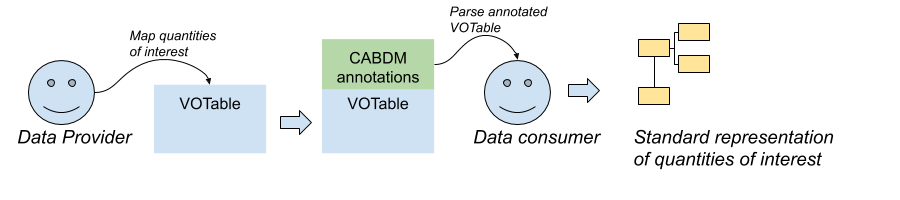
\includegraphics[width=0.9\textwidth]{fig1.png}
\caption{CAB-MSD workflow}
\label{fig:workflow}
\end{figure}


\subsection{Model}

The class diagram of figure \ref{fig:classdiag} shows the coarse components of CAB-MSD. 

\begin{itemize}
    \item A CAB-MSD instance can contains a set of measurements
    \begin{itemize}
        \item The set of CAB-MSD measurements is the same for all instances of a given dataset (VOTable).
        \item The set of measurements is not defined by the model but it is specific to one VOTable
        \item All supported measurements are modeled in CAB-MSD or taken out from imported models.
    \end{itemize}
\item A CAB-MSD instance can contains a set of associated data.
    \begin{itemize}
        \item Other CAB-MSD instances
        \item VO products (e.g. SSLAP response)
        \item Dataset returned by VO services (e.g. Datalinks)
        \item Other VO model instances (e.g. Provenance, DatasetMetaData)
        \item All links have a semantic tag.
    \end{itemize}
\end{itemize}


\begin{figure}
\centering
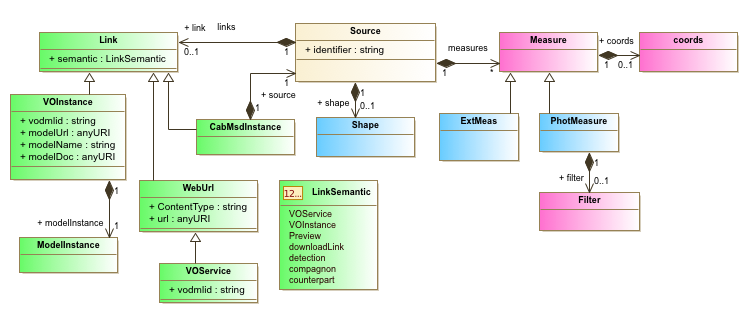
\includegraphics[width=1.0\textwidth]{CABSDM_diagram.png}
\caption{Class diagram}
\label{fig:classdiag}
\end{figure}

Table \ref{table:tclass} gives a few details on the model classes.

\begin{table}[H]
\begin{tabular}{|r|p{19em}|}
  \hline
          \multicolumn{1}{|c}{\bfseries Class} &
          \multicolumn{1}{|c|}{\bfseries Role}
          \\
\hline
Source & 
Root class of the model - just needs a unique identifier
\\  
\hline
Measure & 
Imported from STC2 
\\
\hline
PhotometricMeas & 
Derived from STC2:Meas - connected with PhotDM 
\\
\hline
ExtMeas & 
STC2:Meas extension - Describes usual quantities that are not in STC2  
\\
\hline
Shape & 
Source shape - The way to put shapes in  CAB-
MSD is not given here
\\
\hline
Links & 
Superclass for links - just contains the semantic of the link
\\
\hline
VOInstance & 
Link to an instance of another VO models (e.g. Provenance)
\\
\hline
ModelInstance & 
Container for instances of another VO models (TBD))
\\
\hline
WebUrl & 
Pointer to a Web service 
\\
\hline
VOService & 
Pointer to a VO compliant Web service 
\\
\hline
Cabmsd & 
Pointer to a CAB-MSD instance 
\\
\hline
\end{tabular}
\caption{Table inside a floating element}
\label{table:tclass}
\end{table}

We expect that the use of abstract super-classes will help to build mapping snippets that make easier the annotation job for non model experts.

\subsection{Annotations}

To fulfill the requirements,  CAB-MSD standard should embed its own annotation syntax. 

This proposal is derived from the VO-DML mapping syntax proposed by \citep{wd:wdmapping}:
\begin{itemize}
\item Annotation block separated from the data. Original data are not altered by the mapping, the mapping can work (almost)  whatever the way data are organized.
\item One annotation block per <TABLE>
\item Internal reference based on VO-DML identifiers and on VOTable identifiers.
\item Foreign key mechanism
\end{itemize}

After some tests with time domain data, \cite{talk:lmlite} \cite{talk:lmgaia} proposed some enhancements targeting a better human-readability and an easier job for legacy clients and for legacy data curators.

\begin{itemize}
\item Making the syntax liter anywhere it is possible
\item Using sometime element attributes than specific XML elements to facilitate the templating
\item Implicitly considering that one model instance corresponds to one row of the root table and explicitly indicating that root table.
\end{itemize}

This work could be a solid basis for the CAB-MSD annotation mechanism.

\subsection{Client API}
APIs are not part of the standard, but we could benefit from a common definition of browsing CAB-MSD instances.  This would facilitate the work for developers and improve the interoperability in sense that new features would have to be first applied to a generic interface before to be coded.
Such an interface has been tested with GAIA time series \citep{talk:lmparser}. It is based on selectors using VO-DML identifiers and returning dictionaries (hash maps) rather than (java or Python) class instances. 
The Java snippet below, extracting the first photometric point of a time series, comes from this demonstrator. 

\begin{lstlisting}[language=java]
/*
 * Extract the first photometric point
 */
MappingElement firstPoint = pointList.getContentElement(0);		
List<MappingElement> mesures =
    firstPoint.getSubelementsByRole("meas:CoordMeasure.coord");
/*
 * Measurments of a photometric point are identified by their roles. 
 * To extract time and mag, we have to read all of them and to check the roles
 */
for( MappingElement mes: mesures){
	MappingElement x;
	if( (x = mes.getContentElement("coords:domain.time.JD.date")) != null ) {
		sparseCubeReport.firstTime  = x.getStringValue();
	} else if ( (x = mes.getContentElement("ts:Magnitude.value")) != null ) {
	    sparseCubeReport.firstMag = x.getStringValue();
	} 
}
\end{lstlisting}


\section{Conclusions and Prospects}

This note is not detailed enough to ensure that  CAB-MSD does fulfill all requirements; table \ref{table:tconclusion} show hows this could be achieved by this proposal.

\begin{table}[H]
\begin{tabular}{|p{9em}|p{20em}|}
 \hline
Minimizing the data annotation cost & 
A mapping syntax designed to promote the use of templates
Only the requested quantities are mapped.
\\  
\hline
Flexibility & 
The APIS is based on selectors using VO-DML identifiers (strings passed as function parameters). 
The code has just to build maps with data matching the selector: no model specific code
\\
\hline
Homogeneity & 
All quantities are mapped with the same syntax. The measurement structure (value/frame) is always based on STC.
\\  
\hline
Link support &
Links with different sorts of datasets or services are well supported.
\\ 
\hline
\end{tabular}
\caption{Table inside a floating element}
\label{table:tconclusion}
\end{table}

A large part of the requirements have been issued from the Paris Interop, but the proposed solutions relies on ideas discussed first in the frame of the VO-DML mapping focus group and then within the TDIG. They have been tested and code has been published.
This is why we are confident to have a solid basis for a model for source data. Paying attention to the interest of the community for CAB-MSD, we need now to check, keyboard on the table, that the use cases are really supported by the model, that the annotation process is acceptable and that coding parsers is easy, especially with AstroPy.
This is a big job, thus contributors are welcome. We think it's worth it.

\appendix

\section{TAP response annotation}
\subsection{Storing CAB-MSD instance in a TAP service}
The relational mapping of CAB-MSD is quite straightforward. We have one master table for the Source class and one table for each set of associated data (e.g. compagnons).
In the TAP\_SCHEMA , all UType columns related to the  CAB-MSD stuff can be tagged with CAB-MSD identifiers (VO-DML ids): 
\begin{table}
\begin{tabular}{|p{9em}|p{20em}|}
 \hline
tables & 
Indicates whether the table contains CAB-MSD instances
\\  
\hline
columns &
Indicates CAB-MSD quantity attached to the column
\\
\hline
keys &
Indicates the semantic of the link represented by the join.
Both table must then be declared as CAB-MSD instances
\\  
\hline
\end{tabular}
\caption{Table inside a floating element}
\label{table:ttap}
\end{table}

If the use of Utype columns is conflicting, the TAP service can manage   CAB-MSD identifiers in a private way.

\subsection{Querying CAB-MSD instances}

There are 2 cases here.
\begin{itemize}
    \item If the user just want to query a table as usual, we are in a regular situation. The query engine runs the request and annotates the columns with the Utype columns of the TAP\_SCHEMA whatever their content (model or Utype)
    \item If the user want to get complete CAB-MSD instances, he/she can setup complex query with all needed joins. This works but with 2 major drawbacks:
    \begin{itemize}
        \item The query is quite difficult to write
        \item The result is stacked in one denormalized table difficult to process
    \end{itemize}
\end{itemize}

\section{A proposal to query CAB-MSD instances in one shot}
ADQL is a  tabular oriented query language, thus there is no way to use it to get a set of model components in one shot.
This can be worked around whether the TAP server is informed that the request concerns model instances. It can then trigger right actions.
This notification could done by a specific statement in the SELECT clause. Below is an example of such a hack:
\begin{lstlisting}[language=SQL]
SELECT ivoa.cabmsd FROM master_table WHERE . . . 
\end{lstlisting}
This hides the requested columns and thus makes sure that all model quantities will be returned.
Once the server has understood that CAB-MSD instances are requested, it can run first the query on the master\_table (Source in the model) and then on all the joined tables.
All result tables can be stored in the resulting VOTable and properly mapped by using the models tags from either the TAP\_SCHEMA or the inner mapping template.

This could work in a simple way as long as the WHERE clause is restricted to master\_table. 

\bibliography{myrefs,ivoatex/ivoabib,ivoatex/docrepo}

\end{document}
